\chapter{Hardware Based Security}
Traditional computing has 6 principle regarding processors designes, which are used to enhance the
performces squeezing the most out of the hardware, which are:
\begin{itemize}
  \item \textbf{caching}, which hides consecutive memory access latency
  \item \textbf{pipelining}, which allows to execute multiple instructions at the same time
  \item \textbf{prediction}, chich allows to guess the control flow direction before it is known
  \item \textbf{parallelizing}, which allows to process multiple data at the same time
  \item \textbf{use of indirection},
  \item \textbf{specialization}, which allows to use specific hardware for specific tasks
\end{itemize}
All those measures allow to increase the performances of the processor, but they also introduce
vulnerabilities, which can be exploited by attackers.  This is because they were introduced without
considering security, and they were designed to be fast, not secure.  

Of course, not all the processor are general purpose ones, and some of them are designed to be
secure, providing extra logical isolation for the software running on them. This is the case of 
\textbf{Secure Processor Architectures}, which extend a processor with hardware (and related
software) features for the protection of software. The protected sofware and data is called
\textbf{enclave}, but this can also be the whole operating system or a virtual machine. This is done
because even if we trust som hardware, we cannot trust all the software running on it,
\textit{never}.\\
The isolation measures should also cover all kinds of possible ways to perform a information leak,
of any kind of information, both at the architectural and microarchitectural level, and from any
hardware component, meaning that everything should be untrusted by default.
\begin{boxH}
  A computer system with no secure components nor secure processor architecture considers all the
  components as trusted, which is \textbf{not} a good idea.
\end{boxH}

\begin{figure}[H]
  \centering
  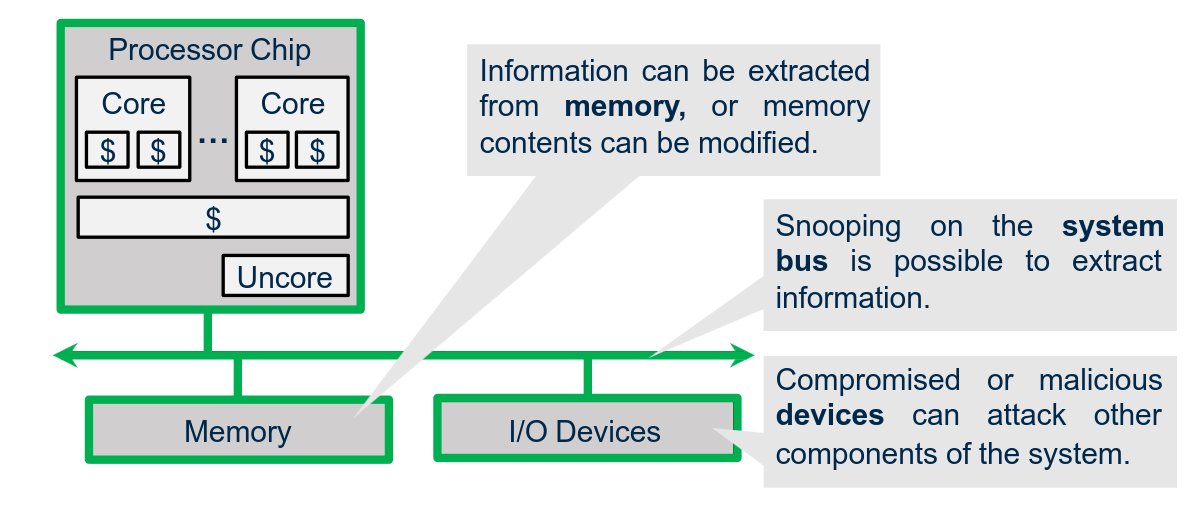
\includegraphics[width=0.7\textwidth]{img/hardware/unsecure processor.png}
  \caption{An example of unsecure processor, with a description of some possible attacks}
\end{figure}

Typically, a computer systen uses a \textbf{ring-based protection scheme}, which gives the most
privileges (and most trust) to the lowest levels of the system software. This means that if the 
lowest level is compromised, the whole system is compromised. Usually, 3 levels are designed:
\begin{itemize}
  \item \textbf{Ring 0}, which is the most privileged level, and is used by the kernel
  \item \textbf{Ring 1 and 1}, which is used by the drivers and other semi-privileged software, but
    it is rarely used
  \item \textbf{Ring 3}, which is used by the applications and us the least privileged level
\end{itemize}
but there are also other levels that can be defined:
\begin{itemize}
  \item \textbf{Ring -1}, which is used by the hypervisor
  \item \textbf{Ring -2}, which is used by the \textbf{System Management Mode} (SMM) and is ussually
    locked down by the processor manifacturer
  \item \textbf{Ring -3}, which is used by the \textbf{Platform management engine} which runs on a
    separate processor
\end{itemize}

\begin{figure}[H]
  \centering
  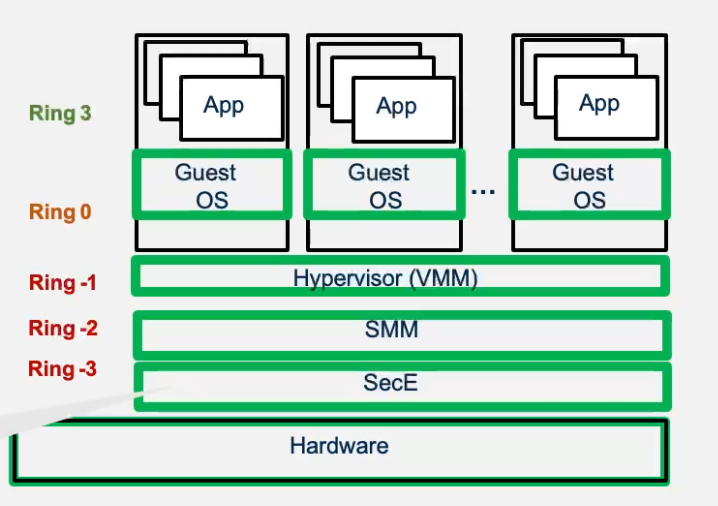
\includegraphics[width=0.5\textwidth]{img/hardware/ring protection scheme.png}
  \caption{The general ring protection scheme}
\end{figure}
In this schema, the relationship between the ring level and the privilege level is inverted, meaning
that the higher the ring level, the lower the privilege level. This schema also guarantees extra
layers of protection to the hardware, which is the most trusted component of the system, but it
instrincaly means that each component trust the lower one.\\
So far we have considered the processor to be secure, which means that we trust it, but the same is
not true for the rest of the hardware, such as the memory or the bus. From those components, threats
can arise, which are \textit{underestimated} when designing a secure processor architecture, part of
those can't even be dealt with in a proper way, for example side channels.
\begin{section}{TEE and TCB}

\end{section}
